The proposed \nep\ development is of sufficient complexity that it is unsurprising that 
in the scientific literature there is a lack of precedent. However, in the gaming world,
it is increasingly common to incorporate physical effects into the software. Indeed,
a significant number of features will be shared with a game engine. 
As illustrated in \Fig{gamestruct}, commonalities include not just ``collisions and
physics", but also a ``platform independence" layer, likely
``Third Party SDKs" (software development kits) and many of the ``core systems". It is notable that
there is a scripting system included for developers, a class  which might include some of the
more technically sophisticated users. Unfortunately, detailed pattern information
is harder to extract from Gregory's textbook~\cite{gregory2},
so that the value of \Fig{gamestruct} lies more in a demonstration
that complexity can be managed using a design which is not only layered, but where
each layer consists of anything up to a dozen different modules. The indicated division of 
relevant layers into modules is also of interest.

\begin{figure}
\centerline{\rotatebox{0}{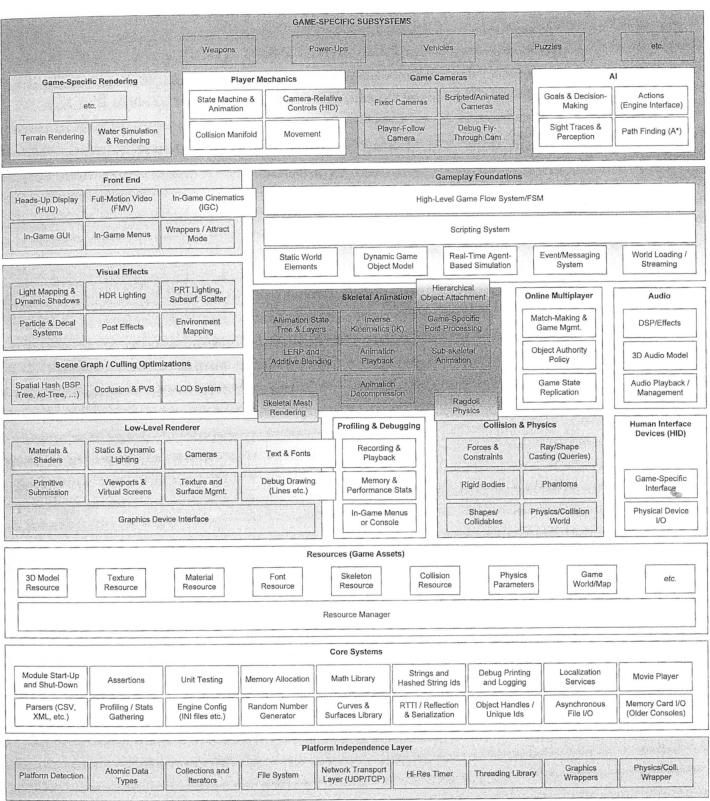
\includegraphics[width=12cm]{../png/game_prog_struct4}}}
\caption{\label{fig:gamestruct}
Diagram illustrating complexity of a game engine, reproduced from Gregory~\protect\cite[\S\,1.6]{gregory2}.}
\end{figure}
